\documentclass[12pt]{article}
\usepackage{graphics}
\usepackage[top=1in,bottom=1in,left=1in,right=1in]{geometry}
\usepackage{alltt}
\usepackage{array}	
\usepackage{graphicx}
\usepackage{tabularx}
\usepackage{verbatim}
\usepackage{setspace}
\usepackage{listings}


\usepackage{amssymb,amsmath, amsthm}
\usepackage{zed-csp}
\usepackage[cc]{titlepic}

\title{SOEN 331 - S: Formal Methods\\for Software Engineering\\
\ \\
Assignment 1}
\author{Nathan Grenier, Nirav Patel}
\date{\today}
\begin{spacing}{1.5}
\begin{document}
\maketitle
\thispagestyle{empty}

\newpage

\pagenumbering{arabic}
							    
\section*{PROBLEM 1: Propositional logic (5 pts)}


You are shown a set of four cards placed on a table, each of which has a \textbf{number} on one
side and a \textbf{color} on the other side. The visible faces of the cards show the numbers \textbf{9} and
\textbf{11}, and the colors \textbf{blue}, and \textbf{yellow}.\\
										
Which card(s) must you turn over in order to test the truth of the proposition that “\textit{If
the face of a card is \textbf{blue}, then it has a \textbf{prime} number on the other side}”? Explain your
reasoning by deciding for \underline{each} card whether or not it should be turned over and why.\\
\textbf{Solution}: 
\\
We're trying to prove the proposition: $$p \rightarrow q$$

\textbf{Where:} 
\begin{itemize}
	\item $p$ represents the proposition that the card is blue, and
	\item $q$ represents the proposition that the other side of the card has a prime number on its face.
\end{itemize}


\begin{enumerate}
	\item \textbf{Blue Card:} You \textbf{should} flip this card to prove the proposition. We can apply modus ponens to the proposition to prove it. This would show that if the card is blue, then the other side has a prime number. 
	\[
	\frac{
	\begin{array}{c}
		p \rightarrow q \\
		p \\
	\end{array}
	}{
	\begin{array}{c}
		\therefore q
	\end{array}
	}
	\]
	\item \textbf{9 Card:} You \textbf{should} flip this card to prove the proposition. We can apply modus tollens to the proposition to prove it. This would show that if the other side of the card is not a prime number, then the card is not blue.
	\[
		\frac{
		\begin{array}{c}
			p \rightarrow q \\
			\neg q \\
		\end{array}
		}{
		\begin{array}{c}
			\therefore \neg p
		\end{array}
		}
		\]
	\item \textbf{Yellow Card:} You \textbf{should not} flip this card to prove the proposition. The proposition in question is only concerned with the blue cards. It makes no assertion about yellow cards. Flipping this card would fall under the category of affirming the consequent, which is not a valid way to prove the proposition.
	\item \textbf{11 Card:} You \textbf{should not} flip this card to prove the proposition. The proposition makes no claim that cards with prime numbers on them must have blue on the other side. This would fall under the category of denying the antecedent which is a logical fallacy.
\end{enumerate}

\pagebreak

\section*{PROBLEM 2: Predicate logic (14 pts)}
												
	\textbf{Part 1} (8 pts)\\
	Consider types \textit{Object}, and the binary relation Orbits over the domain of all celestial objects,
	which is codified by clause \texttt{object/1} in Prolog (available in \texttt{solar.pl}):

	\begin{enumerate}
		\item  (2 pts) Construct a formula in predicate logic to define a planet, where planet is defined
		as an object whose mass is greater than or equal to $0.33 \times 10^{24}KG$, and which it orbits around the sun. For all practical purposes, you may ignore the $10^{24}KG$ factor.

		\textbf{Solution:}
		\begin{itemize}
			\item Let $M(x)$ be that the mass of object $x$ greater than or equal to $0.33 \times 10^{24}KG$.
			\item Let $O(x, y)$ be that $x$ orbits around $y$.
			\item Let $P(x)$ be that $x$ is a planet.
		\end{itemize}

		The formula to define a planet is: $$P(x) \equiv M(x) \land O(x, sun)$$

		Use the formula for Planet to construct a formula that defines the binary relation
		is satellite of in terms of the binary relation Orbits. A satellite is an object that
		orbits around a planet.
		
		\textbf{Solution:}
		\begin{itemize}
			\item Let $S(x, y)$ mean that $x$ is a satellite of $y$.
			\item Let $O(x, y)$ be that $x$ orbits around $y$.
			\item Let $P(x)$ be that $x$ is a planet.
		\end{itemize}
		$$S(x, y) \equiv O(x, y) \land P(y) $$

		\item (3 pts) (PROGRAMMING) Map your formulas to Prolog rules is planet/1, and is satellite of/2, and demonstrate how it works by executing both ground- and non-ground queries. Identify the type of each query.
		\textbf{Solution}:
		Here are the translated prologue rules:
		\begin{enumerate}
			\item \textbf{is\_planet/1}
			\begin{lstlisting}[language=Prolog]
planet(X) :- orbits(X, sun), mass(X, M), M >= 0.33.
			\end{lstlisting}
			\item \textbf{is\_satellite\_of/2}
			\begin{lstlisting}[language=Prolog]
is_satellite_of(X, Y) :- is_planet(Y), orbits(X, Y).		
			\end{lstlisting}
		\end{enumerate}

		\textbf{List of example queries:}
		\begin{itemize}
			\item Query \texttt{?- is\_planet(pluto).}
			\begin{itemize}
				\item Type: Ground Query
				\item Result: \texttt{false}
			\end{itemize}
			\item Query \texttt{?- is\_planet(mars).}
			\begin{itemize}
				\item Type: Ground Query
				\item Result: \texttt{true}
			\end{itemize}
			\item Query \texttt{?- is\_planet(P).}
			\begin{itemize}
				\item Type: Non-Ground Query
				\item Result: \texttt{\newline P = mercury \newline P = venus  \newline P = earth \newline P = mars \newline P = jupiter \newline P = saturn \newline P = uranus \newline P = neptune \newline false}
			\end{itemize}
			\item Query \texttt{?- is\_satellite\_of(moon, Planet).}
			\begin{itemize}
				\item Type: Non-Ground Query
				\item Result: \texttt{\newline Planet = earth \newline false}
			\end{itemize}
			\item Query \texttt{?- is\_satellite\_of(S, mars).}
			\begin{itemize}
				\item Type: Non-Ground Query
				\item Result: \texttt{\newline S = deimos \newline S = phobos \newline false}
			\end{itemize}
		\end{itemize}
		
		\begin{figure}[h]
			\centering
			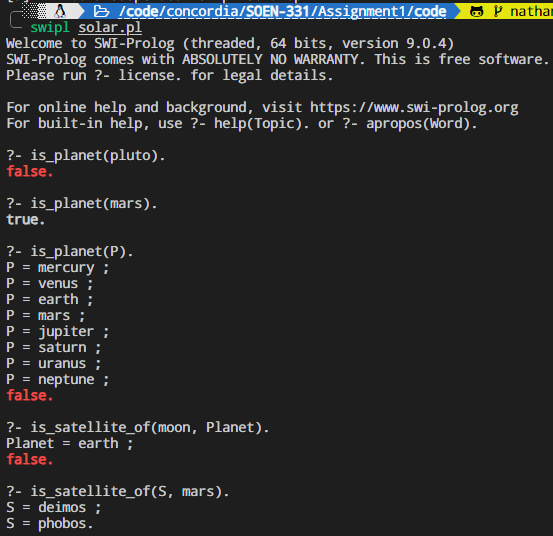
\includegraphics[width=0.7\textwidth]{./static/prolog_queries.png}
			\caption{Screenshot of CLI Outputs}
		\end{figure}
		\item  (3 pts) (PROGRAMMING) Construct a Prolog rule obtain\_all\_satellites/2 that succeeds by returning a collection of all satellites of a given planet.
		
		\textbf{Solution:}
		
		\textbf{obtain\_all\_satellites/2}
		\begin{lstlisting}[language=Prolog, breaklines=true]
obtain_all_satellites(Planet, Satellites) :- findall(Satellite, is_satellite_of(Satellite, Planet), Satellites).
		\end{lstlisting}
	\textbf{List of example queries:}
	\begin{figure}[h]
		\centering
		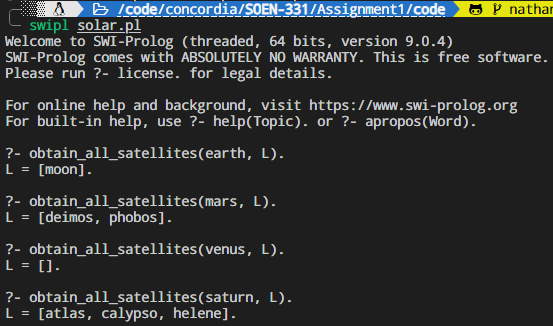
\includegraphics[width=0.7\textwidth]{./static/obtain_all_satellites_query.png}
		\caption{CLI output of the query \texttt{?- obtain\_all\_satellites(earth, Satellites).}}
	\end{figure}
	\end{enumerate}
	
	\noindent \textbf{Part 2: Categorical propositions} (2 pts)\\
	In the domain of all integers, let $number(x)$ denote the statement “$x$ is a number”, and $composite(x)$ denote the statement “$x$ is a composite.” Formalize the following sentences and indicate their corresponding formal type:\\
							
	\textbf{Solution}:
	\begin{enumerate}
		\item "Some numbers are not composite."
		      \begin{itemize}
		      	\item Formalization:
		      	\item Corresponding Formal Type:
		      \end{itemize}
		\item "No numbers are prime."
		      \begin{itemize}
				\item Formalization:
				\item Corresponding Formal Type:
		      \end{itemize}
		\item "Some numbers are not prime."
		      \begin{itemize}
				\item Formalization:
				\item Corresponding Formal Type:
		      \end{itemize}
		\item "All numbers are prime."
		      \begin{itemize}
				\item Formalization:
				\item Corresponding Formal Type:
		      \end{itemize}
	\end{enumerate}
\end{spacing} 
\end{document}
